%!TEX TS-program = xelatex

% Defense presentation based on the official HSE Beamer theme:
% https://www.hse.ru/info/brandbook/

\documentclass[aspectratio=169,10pt]{beamer}

\usepackage{etoolbox}
\newbool{russian}
\booltrue{russian}
\input{hse-theme/hse-beamer-theme.sty}

\usepackage[english,russian]{babel}
\usepackage[no-math]{fontspec}
\IfFontExistsTF{HSE Sans}
  {\setsansfont{HSE Sans}}
  {\setsansfont{Arial}}
\IfFontExistsTF{Arial}
  {\setmainfont{Arial}}
  {\setmainfont{Times New Roman}}
\IfFontExistsTF{Courier New}
  {\setmonofont{Courier New}[Scale=MatchLowercase]}
  {\setmonofont{Menlo}[Scale=MatchLowercase]}

\usepackage{booktabs}
\usepackage{tabularx}
\usepackage{array}
\usepackage{graphicx}
\usepackage{ragged2e}
\usepackage{adjustbox}

\graphicspath{{figures/}}

\newcolumntype{Y}{>{\RaggedRight\arraybackslash}X}
\newcolumntype{Z}{>{\Centering\arraybackslash}X}
\newcolumntype{P}[1]{>{\RaggedRight\arraybackslash}p{#1}}
\newcolumntype{C}[1]{>{\Centering\arraybackslash}p{#1}}
\newcommand{\ms}{\mathrm{ms}}
\newcommand{\smallcell}[1]{\begin{tabular}{@{}c@{}}#1\end{tabular}}
\newcommand{\thead}[1]{\textbf{#1}}
\newcommand{\metric}[2]{%
  \begin{beamercolorbox}[wd=\linewidth,sep=0.65em,center]{BlueOnWhite}
    {\scriptsize\bfseries #1}\\[0.15em]
    {\scriptsize #2}
  \end{beamercolorbox}%
}
\newcommand{\figcap}[1]{%
  \vspace{0.45em}
  \begin{center}
    \begin{minipage}{0.88\linewidth}
      \centering
      {\scriptsize\color{black!68}\linespread{1.18}\selectfont #1\par}
    \end{minipage}
  \end{center}
  \vspace{0.12em}
}
\newcommand{\tightfigcap}[1]{%
  \vspace{0.22em}
  \begin{center}
    \begin{minipage}{0.92\linewidth}
      \centering
      {\scriptsize\color{black!68}\linespread{1.12}\selectfont #1\par}
    \end{minipage}
  \end{center}
  \vspace{-0.02em}
}
\newcommand{\sectionnote}[1]{%
  \vspace{0.25em}
  \begin{center}
    \begin{minipage}{0.88\linewidth}
      \centering
      {\scriptsize\linespread{1.22}\selectfont #1\par}
    \end{minipage}
  \end{center}
  \vspace{0.08em}
}
\newcommand{\aftertablegap}{\vspace{0.90em}}

\setbeamersize{text margin left=0.58cm,text margin right=0.58cm}
\setbeamertemplate{frametitle}{%
  \vspace*{-2.55em}
  \hspace*{1.38cm}%
  \begin{minipage}[t]{0.78\paperwidth}
    \raggedright
    {\usebeamerfont{frametitle}\color{HSEblue}\insertframetitle\par}
    \vspace{0.04em}
    {\usebeamerfont{framesubtitle}\color{black!60}\insertframesubtitle\par}
  \end{minipage}
  \vspace{0.18em}
}
\setbeamertemplate{caption}{\centering\insertcaption\par}
\setbeamerfont{frametitle}{size=\Large,series=\bfseries}
\setbeamerfont{framesubtitle}{size=\footnotesize}
\setbeamerfont{itemize/enumerate body}{size=\footnotesize}
\setbeamerfont{itemize/enumerate subbody}{size=\scriptsize}
\setlength{\tabcolsep}{3pt}
\renewcommand{\arraystretch}{1.13}
\setlength{\leftmargini}{1.25em}

\title[Оптимизация качества облачного видеостриминга]{Оптимизация качества облачного видеостриминга в условиях ограниченности вычислительных ресурсов с применением классических эвристических методов и подходов на основе машинного обучения}
\subtitle{Защита выпускной квалификационной работы}
\author[Д. Д. Паршин]{Даниил Денисович Паршин}
\institute{НИУ ВШЭ, Нижний Новгород\\Факультет информатики, математики и компьютерных наук}
\date{2026}

\begin{document}

\begin{frame}[plain]
  \begin{center}
    
\includegraphics[width=0.085\textwidth]{hse-theme/hse-logo-full-ru}\\[0.45em]
    {\scriptsize НИУ ВШЭ, Нижегородский филиал\\
    Факультет информатики, математики и компьютерных наук}\\[0.75em]
    {\color{HSEblue}\fontsize{11.4}{13.4}\selectfont\bfseries
    Оптимизация качества облачного видеостриминга в условиях ограниченности вычислительных ресурсов с применением классических эвристических методов и подходов на основе машинного обучения\par}
    \vspace{0.65em}
    {\footnotesize Выпускная квалификационная работа - бакалаврская работа}\\[0.85em]
  \end{center}
  \begin{columns}[T,onlytextwidth]
    \column{0.33\textwidth}
      \centering{\footnotesize Студент\\\textbf{Даниил Денисович Паршин}}
    \column{0.33\textwidth}
      \centering{\footnotesize Руководитель\\\textbf{П. А. Колданов}}
    \column{0.33\textwidth}
      \centering{\footnotesize Консультант\\\textbf{В. Г. Жислина}}
  \end{columns}
  \vfill
  \begin{center}{\footnotesize Нижний Новгород, 2026}\end{center}
\end{frame}

\begin{frame}
\frametitle{Проблема}
\framesubtitle{Пространственное распределение качества не определяется только битрейтом}
\footnotesize
\begin{columns}[T,onlytextwidth]
  \column{0.51\textwidth}
  \begin{itemize}
    \item В облачном видеоконвейере CPU-бюджет распределяется между ROI-детекцией, кодированием, сетевым стеком и управляющей логикой.
    \item ABR регулирует потоковые параметры во времени: битрейт, разрешение и профиль. Пространственный приоритет областей внутри кадра при этом не задается.
    \item Перцептивная значимость ошибок неоднородна: деградация текста, лиц и высокочастотных фактур критичнее деградации фоновых областей.
  \end{itemize}
  \column{0.45\textwidth}
  \begin{table}
  \scriptsize
  \begin{tabularx}{\linewidth}{@{}P{0.25\linewidth}Y@{}}
    \toprule
    \thead{ROI-класс} & \thead{Кодировочная роль} \\
    \midrule
    Text & сохранение читаемости UI, субтитров и документов \\
    \addlinespace[0.12em]
    Face & защита субъективно значимых человеческих областей \\
    \addlinespace[0.12em]
    Cloth & снижение артефактов квантования на высокочастотных фактурах \\
    \addlinespace[0.12em]
    Background & источник битового бюджета для перераспределения качества \\
    \bottomrule
  \end{tabularx}
  \end{table}
  \aftertablegap
  \begin{block}{Проблема работы}
    Требуется сформировать для кодировщика пространственный управляющий сигнал без выхода за CPU-бюджет и без существенного роста размера потока.
  \end{block}
\end{columns}
\end{frame}

\begin{frame}
\frametitle{Конкретная задача}
\framesubtitle{Верифицируется контур «ROI-детекция $\rightarrow$ политика кодировщика $\rightarrow$ метрики качества»}
\footnotesize
\begin{columns}[T,onlytextwidth]
  \column{0.45\textwidth}
  \begin{block}{Вклад ВКР}
    \begin{itemize}
      \item ROI-aware оптимизация формализуется как ограниченная задача качества с учетом задержки, битрейта и площади ROI.
      \item IDet рассматривается как CPU-ориентированный слой между моделями компьютерного зрения и политикой кодировщика.
      \item Эффект проверяется через baseline и ROI-aware HEVC при сопоставимом размере выходного потока.
    \end{itemize}
  \end{block}
  \column{0.52\textwidth}
  \begin{table}
  \scriptsize
  \begin{tabularx}{\linewidth}{@{}P{0.28\linewidth}Y@{}}
    \toprule
    \thead{Компонент} & \thead{Назначение в проверке} \\
    \midrule
    p99 $<10\,\ms$ & контроль хвоста распределения задержки \\
    \addlinespace[0.12em]
    size ratio $\approx1$ & исключение выигрыша за счет роста файла \\
    \addlinespace[0.12em]
    area budget & ограничение доли кадра под защитой ROI \\
    \addlinespace[0.12em]
    \texttt{qoffset} & смещение квантования для защищаемой области \\
    \addlinespace[0.12em]
    ONNX artifact & CPU-путь без Python-стека и GPU \\
    \bottomrule
  \end{tabularx}
  \end{table}
  \aftertablegap
  \begin{alertblock}{Область применимости вывода}
    Покадровый эксперимент изолирует пространственный эффект ROI side data; временная стабильность, GOP-динамика и end-to-end latency требуют отдельной видеоверификации.
  \end{alertblock}
\end{columns}
\end{frame}

\begin{frame}
\frametitle{Обзор подходов}
\framesubtitle{Метрики детектора недостаточны для оценки кодировочного эффекта}
\scriptsize
\begin{adjustbox}{max width=\linewidth}
\begin{tabularx}{0.97\linewidth}{@{}P{0.20\linewidth}Y Y@{}}
  \toprule
  \thead{Методический класс} & \thead{Роль в системе} & \thead{Ограничение для данной задачи} \\
  \midrule
  ABR / rate adaptation &
  Регулирует битрейт, разрешение и профиль кодирования на временной шкале потока. &
  Не задает пространственный приоритет и распределение квантизации внутри отдельного кадра. \\
  \addlinespace[0.25em]
  Global PSNR/SSIM/VMAF &
  Дают агрегированную оценку кодека и регрессионного качества. &
  Усредняют ошибки по площади кадра; локальная деградация ROI может быть замаскирована фоном. \\
  \addlinespace[0.25em]
  ROI-/saliency-кодирование &
  Передает кодировщику пространственный управляющий сигнал. &
  Требует устойчивого выделения ROI, area cap, \texttt{qoffset}-policy и временной стабильности. \\
  \addlinespace[0.25em]
  mAP детектора &
  Валидирует ML-компонент на уровне распознавания областей. &
  Не учитывает стоимость CPU-исполнения, p99-задержку, постобработку и фактический эффект в \texttt{libx265}. \\
  \bottomrule
\end{tabularx}
\end{adjustbox}
\vspace{0.55em}
\begin{block}{Методическая позиция ВКР}
Единицей оценки является системный контур: ROI-детекция формирует side data, кодировщик перераспределяет биты, а метрики фиксируют локальный эффект при практически неизменном размере потока.
\end{block}
\end{frame}

\begin{frame}
\frametitle{Предлагаемый подход}
\framesubtitle{Разделение слоя инференса и политики кодировщика}
\footnotesize
\begin{center}
  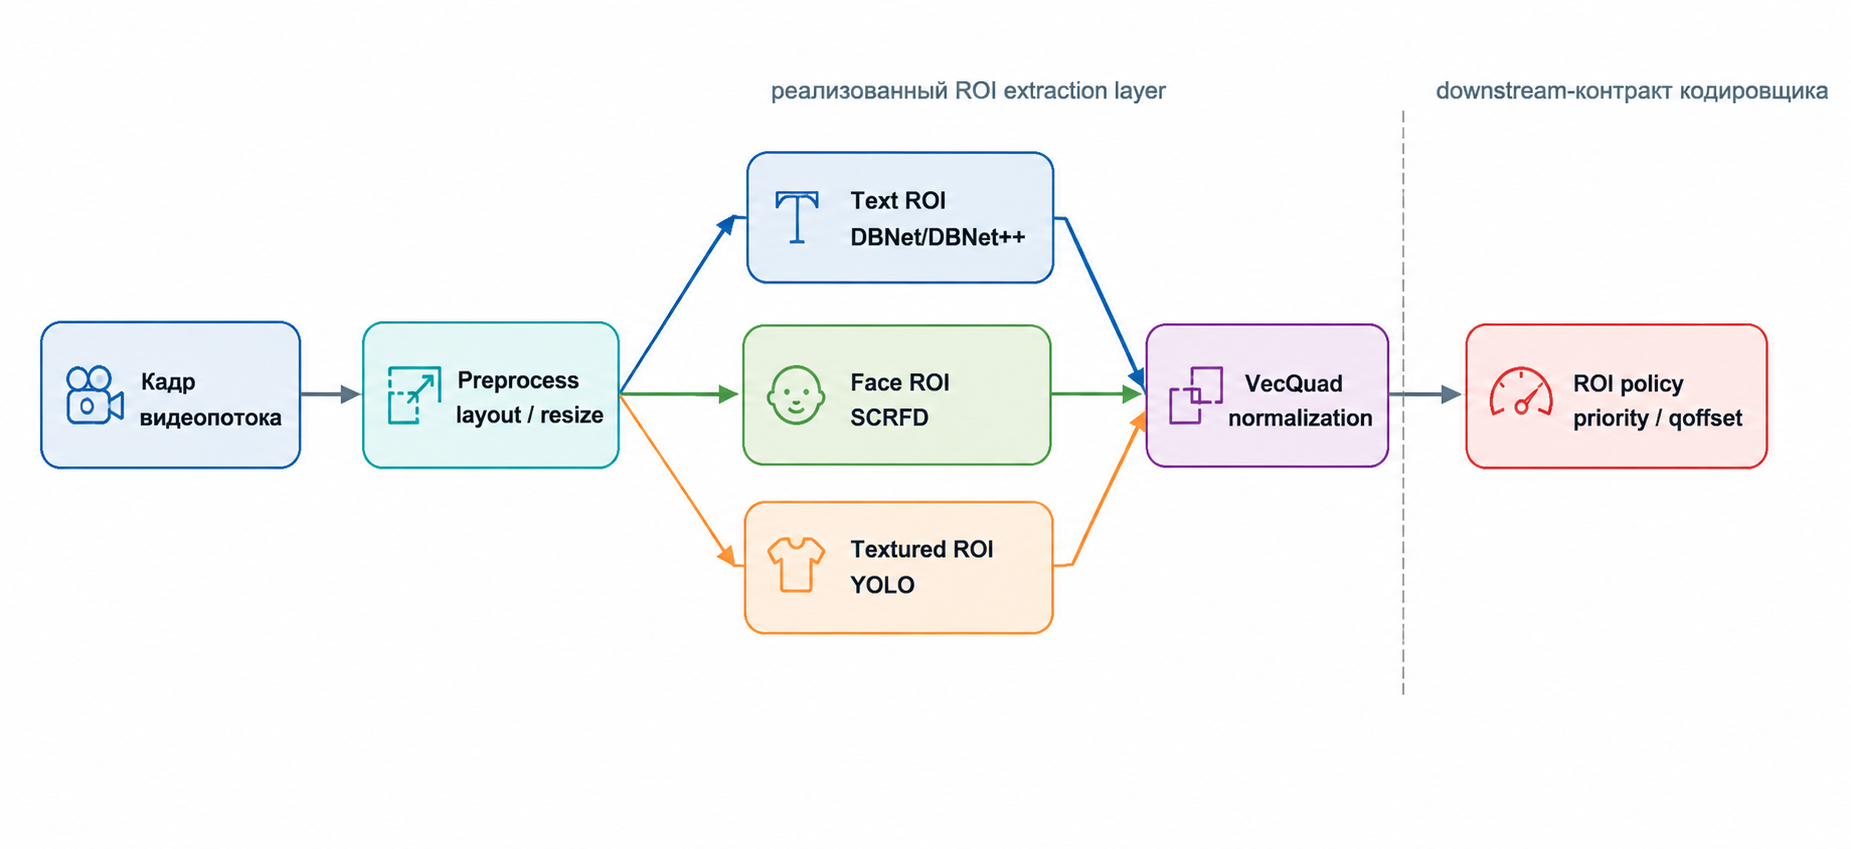
\includegraphics[width=0.82\linewidth,trim=0 58 0 62,clip]{architecture/roi_pipeline_overview.png}
\end{center}
  \tightfigcap{IDet возвращает нормализованную геометрию ROI; кодировочный слой интерпретирует ее как типизированные ROI side data с приоритетом, бюджетом площади и \texttt{qoffset}.}
\sectionnote{\textbf{Граница ответственности:} публичный API IDet остается геометрическим \texttt{VecQuad}; тип, приоритет и \texttt{qoffset} относятся к последующему слою интеграции с кодировщиком.}
\end{frame}

\begin{frame}
\frametitle{Детектор фактурных ROI}
\framesubtitle{Выбор модели определяется стоимостью развертывания, а не только mAP}
\scriptsize
\begin{center}
  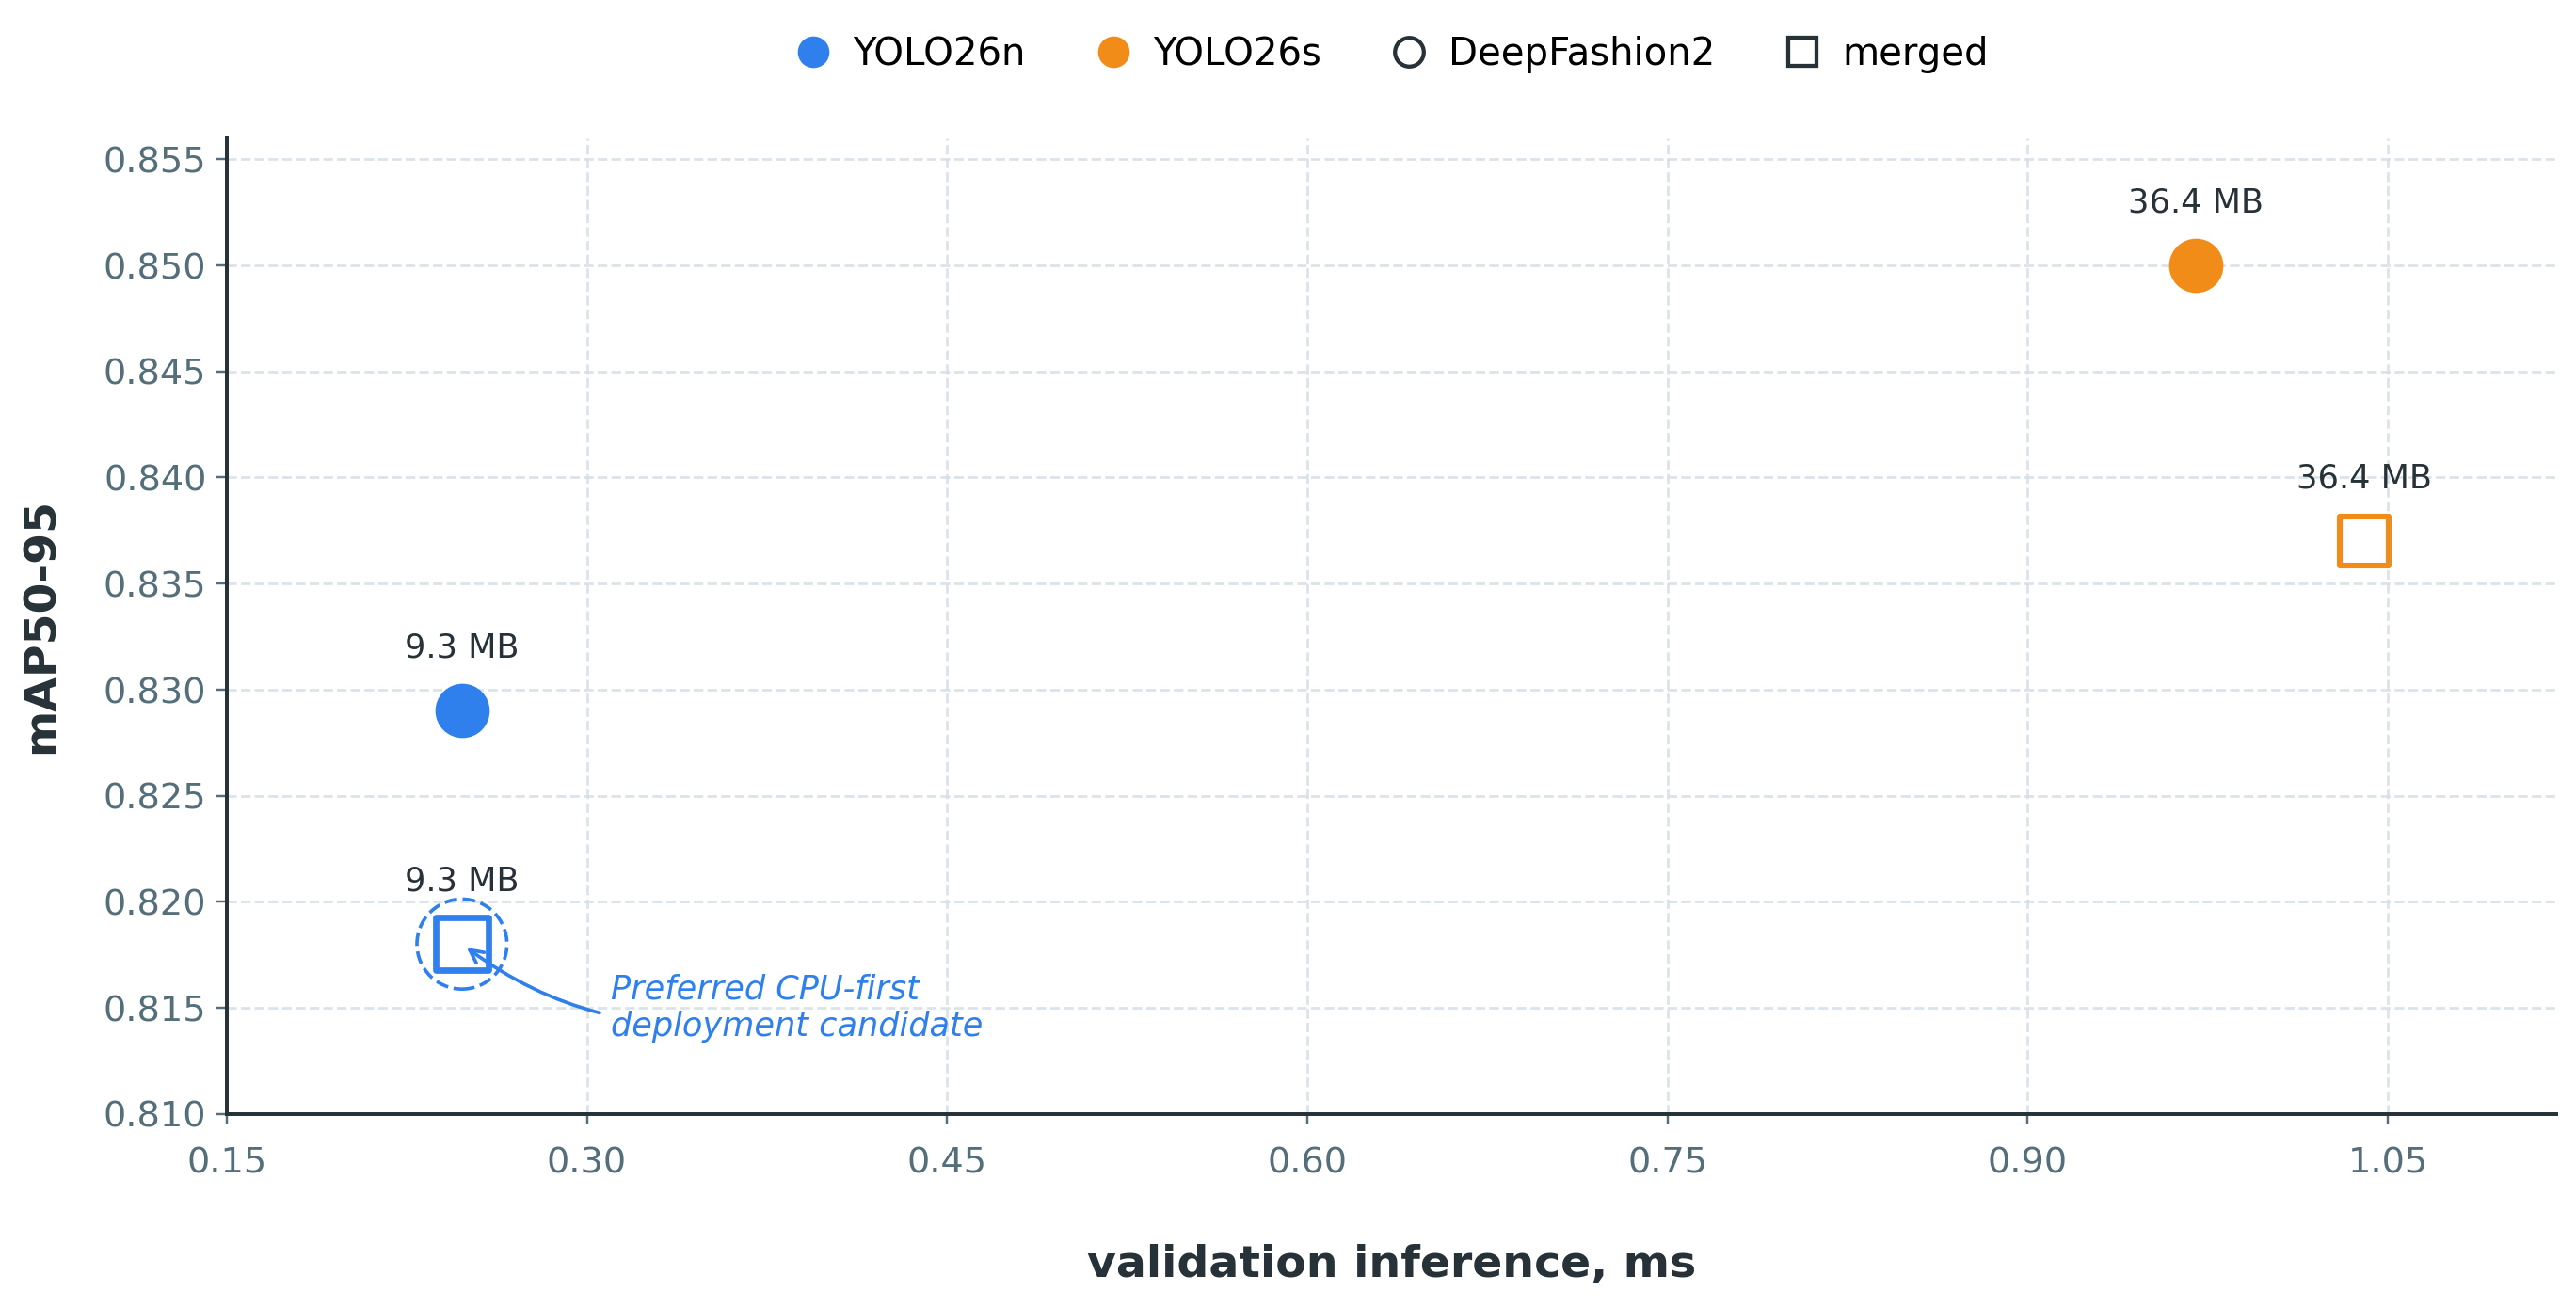
\includegraphics[width=0.75\linewidth]{yolo/yolo_quality_cost_tradeoff.png}
\end{center}
  \tightfigcap{YOLO26n выбран как кандидат для развертывания: 0.818 mAP50-95, 5.2 GFLOPs, 9.3 MB; YOLO26s дает 0.837, но требует 20.5 GFLOPs и 36.4 MB. Данные DeepFashion2 + Fashionpedia сведены к 7 классам; проверены разбиения, bbox и PT-to-ONNX контракт.}
\end{frame}

\begin{frame}
\frametitle{CPU-исполнение IDet}
\framesubtitle{Рабочая точка выбирается по p99 и качеству покрытия ROI}
\scriptsize
\begin{columns}[T,onlytextwidth]
  \column{0.60\textwidth}
  \begin{center}
    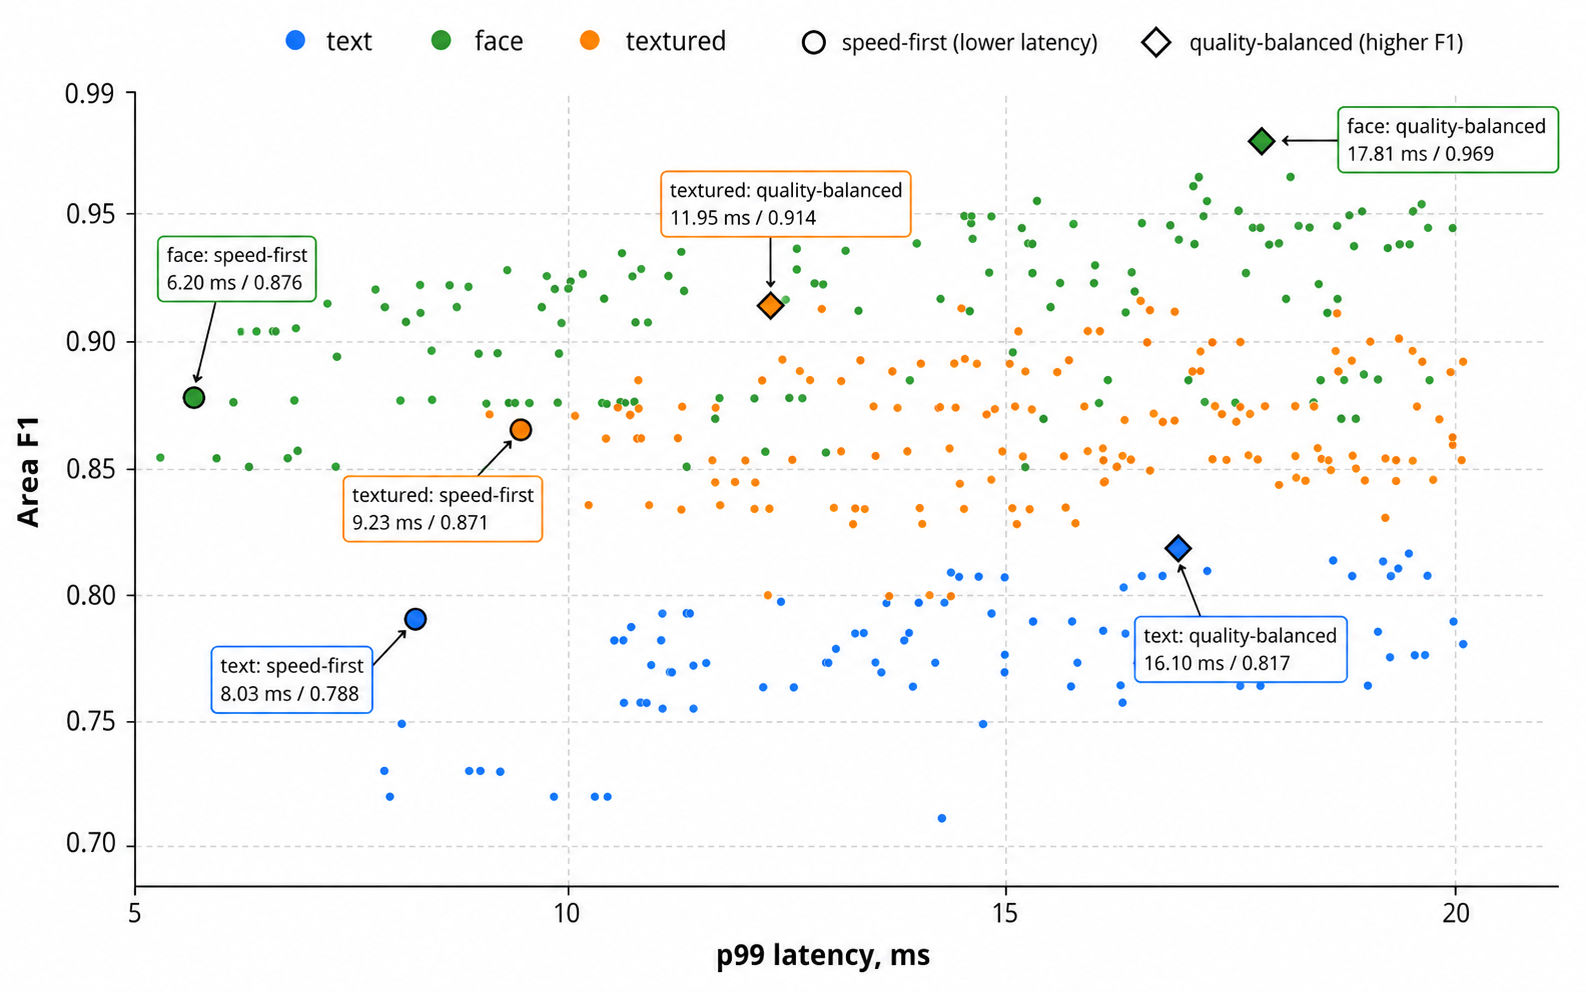
\includegraphics[width=0.95\linewidth]{performance/p99_area_f1_tradeoff.png}
  \end{center}
  \vspace{0.18em}
  {\centering\begin{minipage}{0.88\linewidth}
    \centering{\scriptsize\color{black!68}\linespread{1.15}\selectfont Каждая точка соответствует одной runtime-конфигурации grid-search.\par}
  \end{minipage}\par}
  \column{0.37\textwidth}
  \begin{tabularx}{\linewidth}{@{}P{0.22\linewidth}ZZZ@{}}
    \toprule
    \thead{Режим} & \thead{p99, ms} & \thead{Recall} & \thead{Area F1} \\
    \midrule
    Text & 8.032 & 0.886 & 0.788 \\
    Face & 7.553 & 0.916 & 0.922 \\
    Cloth & 9.230 & 0.920 & 0.871 \\
    \bottomrule
  \end{tabularx}
  \vspace{0.95em}
  \begin{itemize}
    \item p99 измеряется на чистом пути исполнения: без сохранения артефактов, визуализации и диагностического вывода.
    \item Рабочие точки различаются по цене ошибки: Text приоритизирует recall, Face --- Area F1, Cloth ограничен стоимостью YOLO-инференса.
    \item Полный видеоконвейер требует планировщика частоты запусков и переиспользования ROI между кадрами.
  \end{itemize}
\end{columns}
\end{frame}

\begin{frame}
\frametitle{Интеграция ROI в кодировщик}
\framesubtitle{Режим match\_baseline фиксирует сопоставимый размер потока}
\scriptsize
\begin{columns}[T,onlytextwidth]
  \column{0.60\textwidth}
  \begin{center}
    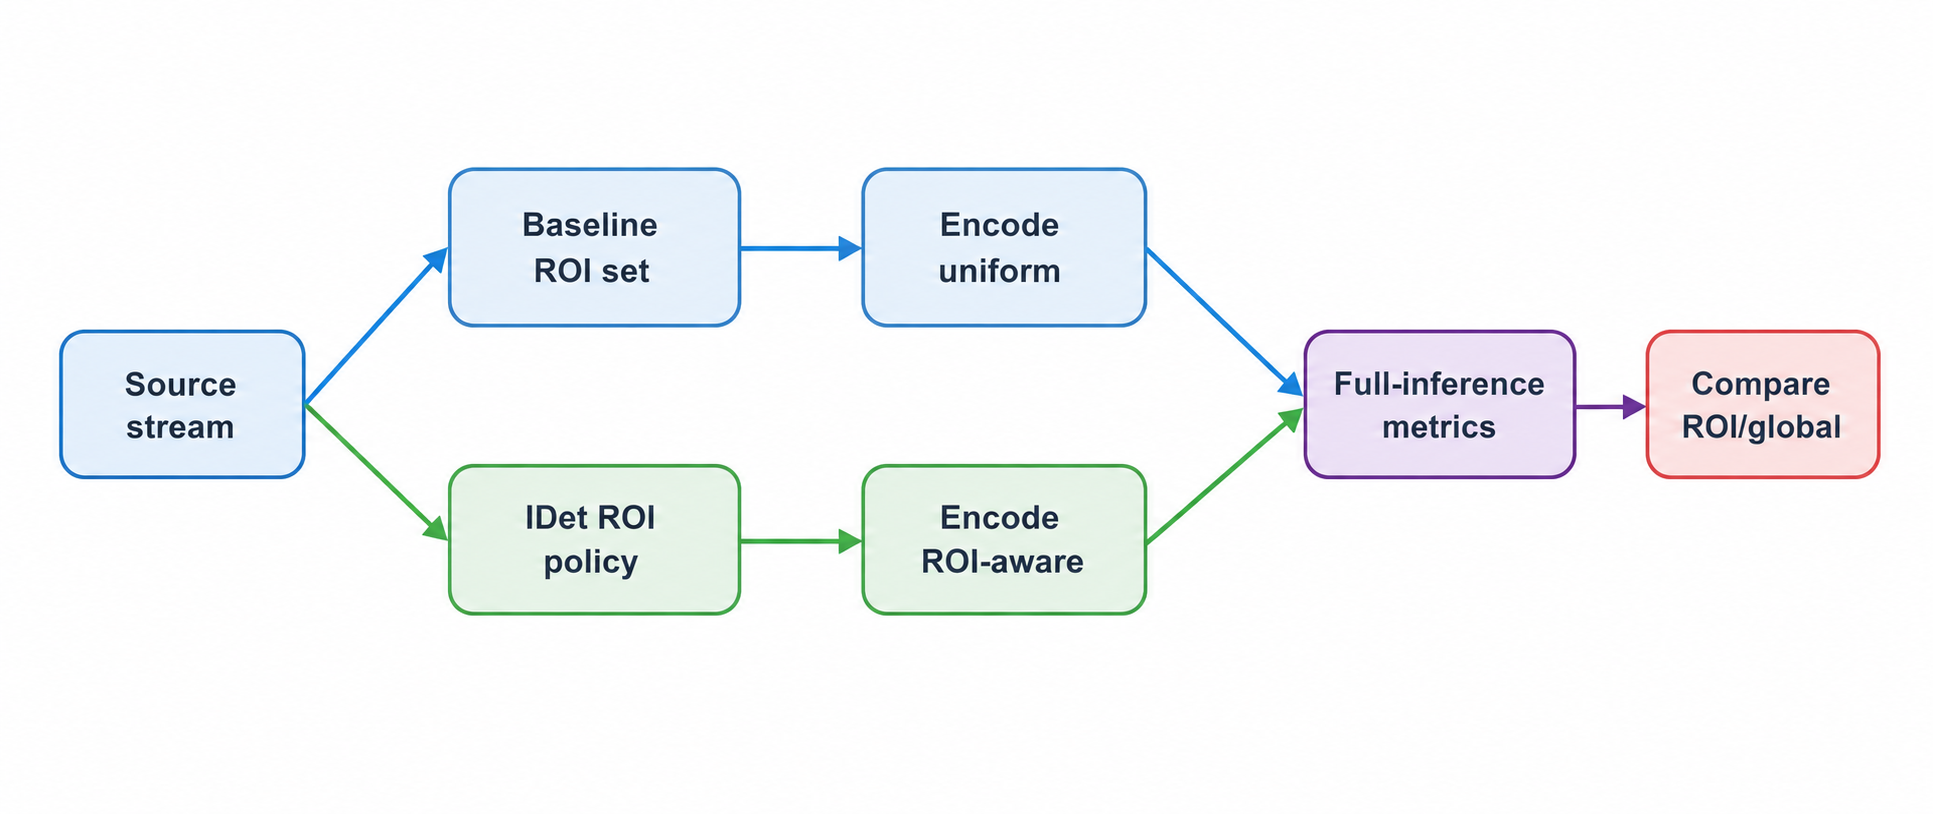
\includegraphics[width=\linewidth,trim=0 120 0 120,clip]{video-quality/roi_encoding_protocol.png}
  \end{center}
  \figcap{Baseline и ROI-aware ветки декодируются в PNG-последовательность и сравниваются с исходными FHD-кадрами.}
  \column{0.37\textwidth}
  \scriptsize
  \begin{tabularx}{\linewidth}{@{}P{0.17\linewidth}ZZZZ@{}}
    \toprule
    \thead{Режим} & \thead{Кадры} & \thead{CRF} & \thead{Ratio} & \thead{qoff.} \\
    \midrule
    Text & 3000 & CRF 32 & 1.0036 & $-1/4$ \\
    Face & 3000 & CRF 32 & 1.0058 & $-1/5$ \\
    Cloth & 2696 & CRF 32 & 1.0029 & $-1/10$ \\
    \bottomrule
  \end{tabularx}
  \vspace{1.00em}
  {\scriptsize\linespread{1.18}\selectfont HEVC: \texttt{libx265}, preset \texttt{medium}. Baseline кодируется без ROI side data; ROI-aware ветка получает \texttt{AVRegionOfInterest} через \texttt{addroi}.\par}
\end{columns}
\sectionnote{Global агрегирует весь кадр, ROI-crop измеряет защищаемую область, Background оценивает цену перераспределения качества при фиксированном размере потока.}
\end{frame}

\begin{frame}
\frametitle{Результаты: локальное качество ROI}
\framesubtitle{Наибольший выигрыш наблюдается для Text и Face ROI}
\scriptsize
\begin{center}
  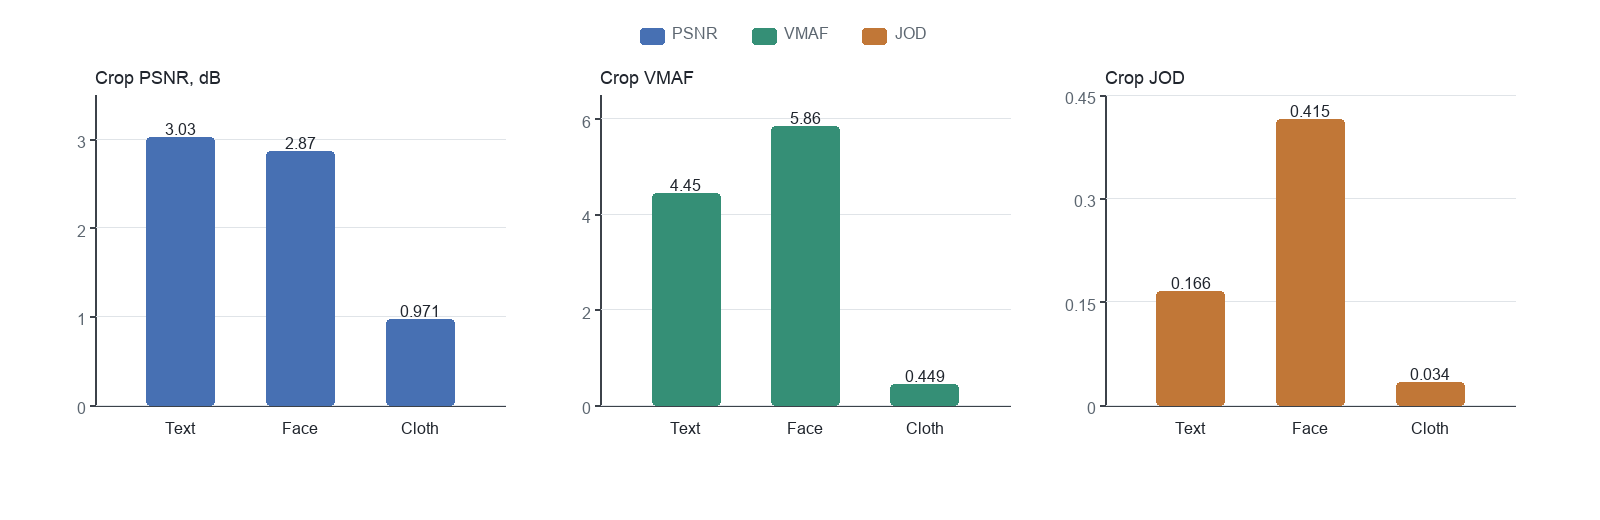
\includegraphics[width=0.92\linewidth]{video-quality/roi_crop_effects.png}
\end{center}
\figcap{ROI-crop improvement: качество измеряется внутри локализованных областей интереса, а не усредняется по всей площади кадра.}
\sectionnote{\textbf{Основной результат:} Text +3.331 dB / +4.451 VMAF; Face +3.284 dB / +5.857 VMAF; Cloth +0.547 dB / +0.449 VMAF. Доля положительных наблюдений: 0.90--1.00.}
\end{frame}

\begin{frame}
\frametitle{Результаты: эффект перераспределения}
\framesubtitle{Фоновая деградация является ожидаемой ценой фиксированного битового бюджета}
\scriptsize
\begin{center}
  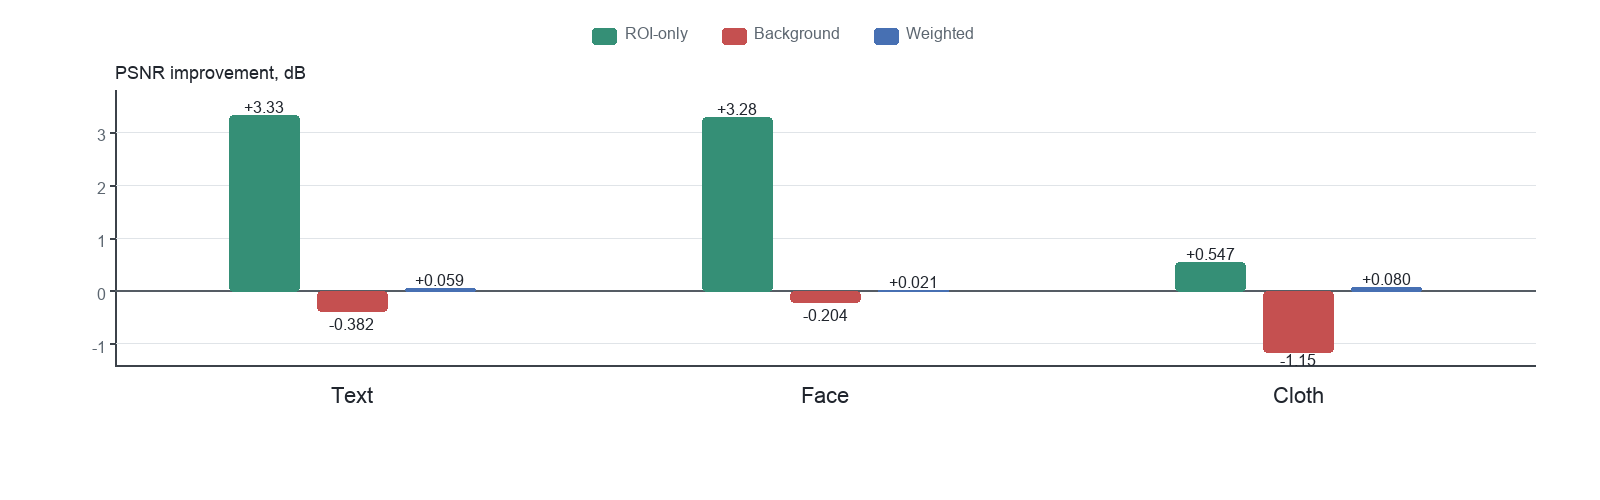
\includegraphics[width=0.92\linewidth]{video-quality/roi_background_tradeoff.png}
\end{center}
\figcap{Рост ROI-only PSNR сопровождается снижением background PSNR, что соответствует перераспределению качества при фиксированном размере.}
\sectionnote{\textbf{Интерпретация:} global/background-метрики фиксируют цену перераспределения, однако ROI-weighted PSNR остается положительным для всех трех типов ROI.}
\end{frame}

\begin{frame}
\frametitle{Ограничения и дальнейшая работа}
\framesubtitle{Верифицированный контур и границы переноса на потоковое видео}
\footnotesize
\begin{columns}[T,onlytextwidth]
  \column{0.48\textwidth}
  \begin{block}{Верифицировано}
    \begin{itemize}
      \item IDet формирует ROI в CPU-бюджете отдельных веток.
      \item YOLO26n выбран как легкая модель для textured ROI.
      \item \texttt{addroi}/\texttt{libx265} дает локальный выигрыш на FHD-кадрах.
      \item Size ratio около 1.0 исключает рост потока как источник выигрыша.
    \end{itemize}
  \end{block}
  \column{0.49\textwidth}
  \begin{alertblock}{За пределами покадрового эксперимента}
    \begin{itemize}
      \item сглаживание и tracking ROI во времени;
      \item GOP-aware настройка межкадрового предсказания;
      \item сквозная latency live-контура с кодировщиком и сетью;
      \item планировщик запуска трех ROI-веток;
      \item I/O Binding и NUMA-настройки на целевой инфраструктуре.
    \end{itemize}
  \end{alertblock}
  \begin{block}{Следующий шаг}
    Проверить на видеокорпусе: стабильность ROI, мерцание качества, битрейт, задержку и сравнение с промышленным baseline.
  \end{block}
\end{columns}
\end{frame}

\begin{frame}
\frametitle{Финальный вывод}
\framesubtitle{Что доказано работой}
\small
  \begin{center}
    \begin{minipage}{0.88\linewidth}
      \centering
	      Работа верифицирует воспроизводимый путь от аудита датасетов и ML-детектора к CPU-исполнению, ROI side data и HEVC-кодированию.
		      ROI-aware слой не заменяет ABR и rate-control, а вводит дополнительный пространственный управляющий сигнал для перераспределения битового бюджета.
    \end{minipage}
  \end{center}
  \vspace{0.9em}
  \begin{columns}[T,onlytextwidth]
    \column{0.31\textwidth}
			      \metric{Исполнение}{IDet формирует ROI-геометрию в CPU-бюджете и сохраняет границу API.}
    \column{0.31\textwidth}
			      \metric{Выбор модели}{YOLO26n выбран после аудита данных, mAP/GFLOPs анализа и ONNX-экспорта.}
    \column{0.31\textwidth}
			      \metric{Кодирование}{ROI-aware HEVC дает локальный выигрыш при size ratio около 1.0.}
  \end{columns}
  \vspace{1.0em}
	  \begin{alertblock}{Итоговый тезис}
	    Подтвержден не глобальный рост качества, а управляемый локальный выигрыш ROI при фиксированной HEVC-конфигурации и сопоставимом размере потока.
  \end{alertblock}
\end{frame}

\begin{frame}[plain]
  \begin{center}
    \vspace{1.2em}
    
\includegraphics[width=0.15\textwidth]{hse-theme/hse-logo-mark}\\[1.2em]
    {\color{HSEblue}\fontsize{25}{29}\selectfont\bfseries Спасибо за внимание}\\[0.9em]
    {\large Готов ответить на вопросы}\\[2.0em]
  \end{center}
\end{frame}

\end{document}
